\documentclass{scrartcl}
\usepackage{graphicx,amsmath,latexsym}
\usepackage{color,psfrag,boxedminipage,amssymb}
%\usepackage[latin1]{inputenc}
%\usepackage[swedish]{babel}
%\usepackage{draftcopy}
\usepackage{tikz}
\usepackage{pgf}
\usetikzlibrary{positioning,arrows}

\newcommand{\st}{\ensuremath{\boldsymbol{s}_k(\boldsymbol{\theta})}}
\newcommand{\St}{{\mathbf S}\ensuremath{(\boldsymbol{\theta})}}
\newcommand{\phibf}{\ensuremath{\boldsymbol{\phi}}}
\newcommand{\varphibf}{\ensuremath{\boldsymbol{\varphi}}}
\def \phibfh{\ensuremath{\hat{\boldsymbol{\phi}}}}
\renewcommand{\sp}{\ensuremath{\boldsymbol{s}(\boldsymbol{\phi})}}
\newcommand{\hp}{\ensuremath{\boldsymbol{h}(\boldsymbol{\phi})}}
\newcommand{\thk}{\ensuremath{\boldsymbol{\theta}_k}}
\renewcommand{\th}{\ensuremath{\boldsymbol{\theta}}}
\newcommand{\alp}{\ensuremath{\boldsymbol{\alpha}}}
\def \thh{\ensuremath{\hat{\boldsymbol{\theta}}}}
\def \epsbf{\ensuremath{\boldsymbol{\epsilon}}}
\def \tht{\tilde{\th}}
\newcommand{\mubf}{\ensuremath{\boldsymbol{\mu}}}

\newcommand{\ctft}{\buildrel{{\cal F}}\over{\longleftrightarrow}}
\newcommand{\defin}{\buildrel{\triangle}\over{=}}

\def \Em{{\mathbb{E}}}



\def \abf{{\mathbf a}}
\def \Abf{{\mathbf A}}
\def \bbf{{\mathbf b}}
\def \Bbf{{\mathbf B}}
\def \cbf{{\mathbf C}}
\def \Cbf{{\mathbf C}}
\def \dbf{{\mathbf d}}
\def \Dbf{{\mathbf D}}
\def \ebf{{\mathbf e}}
\def \Ebf{{\mathbf E}}
\def \fbf{{\mathbf f}}
\def \Fbf{{\mathbf F}}
\def \gbf{{\mathbf g}}
\def \Gbf{{\mathbf G}}
\def \hbf{{\mathbf h}}
\def \Hbf{{\mathbf H}}
\def \ibf{{\mathbf i}}
\def \Ibf{{\mathbf I}}
\def \jbf{{\mathbf j}}
\def \Jbf{{\mathbf J}}
\def \kbf{{\mathbf k}}
\def \Kbf{{\mathbf K}}
\def \lbf{{\mathbf l}}
\def \Lbf{{\mathbf L}}
\def \mbf{{\mathbf m}}
\def \Mbf{{\mathbf M}}
\def \nbf{{\mathbf n}}
\def \Nbf{{\mathbf N}}
\def \obf{{\mathbf o}}
\def \Obf{{\mathbf O}}
\def \pbf{{\mathbf p}}
\def \Pbf{{\mathbf P}}
\def \qbf{{\mathbf q}}
\def \Qbf{{\mathbf Q}}
\def \rbf{{\mathbf r}}
\def \Rbf{{\mathbf R}}
\def \sbf{{\mathbf s}}
\def \Sbf{{\mathbf S}}
\def \tbf{{\mathbf t}}
\def \Tbf{{\mathbf T}}
\def \ubf{{\mathbf u}}
\def \Ubf{{\mathbf U}}
\def \vbf{{\mathbf v}}
\def \Vbf{{\mathbf V}}
\def \wbf{{\mathbf w}}
\def \Wbf{{\mathbf W}}
\def \xbf{{\mathbf x}}
\def \Xbf{{\mathbf X}}
\def \ybf{{\mathbf y}}
\def \Ybf{{\mathbf Y}}
\def \zbf{{\mathbf z}}
\def \Zbf{{\mathbf Z}}
\def \0bf{{\mathbf 0}}

\def \Emean{\mathbb{E}}

\def \Sibf{{\mathbf \Sigma}}
\def \xbbf{\mathbf{\bar{x}}}
\def \etr{\mbox{etr}}
\def \tr{\mbox{tr}}
\def \Tr{\mbox{Tr}}
\def \Cov{\mbox{Cov}}
\def \cost{\mbox{cost}}
\def \diag{\mbox{diag}}
\def \Lambf{{\mathbf{\Lambda}}}
\def \Gambf{{\mathbf{\Gamma}}}
\def \Sigbf{{\mathbf \Sigma}}
\newcommand{\rhobf}{\ensuremath{\boldsymbol{\rho}}}
\newcommand{\lambf}{\ensuremath{\boldsymbol{\lambda}}}
\newcommand{\nubf}{\ensuremath{\boldsymbol{\nu}}}

\newcounter{examplenr}[section]
\renewcommand{\theexamplenr}{\arabic{examplenr}}%{\thesection.\arabic{examplenr}}
\newenvironment{example}[1]{\vskip \baselineskip
\refstepcounter{examplenr}\noindent{{\bf
Example~\theexamplenr}\hskip .5em #1\\} }{\hrulefill $\Box$
 \vskip\baselineskip}



\newcounter{theoremnr}[section]
%\renewcommand{\thetheoremnr}{\thesection.\arabic{theoremnr}}
\renewcommand{\thetheoremnr}{\arabic{theoremnr}}
\newtheorem{A}[theoremnr]{Theorem}
\newcounter{theoremProofnr}[section]
%\renewcommand{\thetheoremProofnr}{\thesection.\arabic{theoremProofnr}}
\renewcommand{\thetheoremProofnr}{\arabic{theoremProofnr}}
\newtheorem{B}[theoremProofnr]{Proof of Theorem}
\newcounter{corollarynr}[section]
\renewcommand{\thecorollarynr}{\thesection.\arabic{corollarynr}}
\newtheorem{C}[corollarynr]{Corollary}
\newcounter{Lemmanr}[section]
\renewcommand{\theLemmanr}{\thesection.\arabic{Lemmanr}}
\newtheorem{D}[Lemmanr]{Lemma}
\newcounter{LemmaProofnr}[section]
\renewcommand{\theLemmaProofnr}{\thesection.\arabic{LemmaProofnr}}
\newtheorem{E}[LemmaProofnr]{Proof of Lemma}

\newcounter{propositionnr}[section]
\renewcommand{\thepropositionnr}{\arabic{propositionnr}}
\newtheorem{F}[propositionnr]{Proposition}
\newcounter{propositionProofnr}[section]
\renewcommand{\thepropositionProofnr}{\arabic{propositionProofnr}}
\newtheorem{G}[propositionProofnr]{Proof of proposition}

\newenvironment{working}{\color{blue}\sffamily\em}{}
\newenvironment{forslag}{\color{red}\sffamily\em}{}

\newcounter{definnr}[section]
\renewcommand{\thedefinnr}{\arabic{definnr}}
\newtheorem{J}[definnr]{Definition}



\usepackage{amsmath}
\usepackage{geometry}
\usepackage{caption}
\usepackage{lipsum}
\usepackage{hhline}
\geometry{a4paper}
% \usepackage[backend=biber,style=ieee]{biblatex}
% \addbibresource{ref.bib}
\usepackage{comment}
\usepackage{multirow,array,units}

\usepackage{fancyhdr}

\pagestyle{fancy}
\fancyhf{}
\lhead{Web Science}
\rhead{Assignment 1}

\newenvironment{redmatrix}
  {\left(\array{@{}rrr|ccc@{}}}
  {\endarray\right)}
\newenvironment{ropmatrix}
  {\array{@{}c@{}}}
  {\endarray}
\newcommand\opone[2]{\xrightarrow{(#1)\times r_#2}}
\newcommand\optwo[3]{\xrightarrow{r_#1{}+{} #2r_#3}}
\begin{document}
\title{Web Science Assignment 1}
\subtitle{Movie Recommendation}
\maketitle

\section{}
The aim of the project is to construct a movie recommender given the 100k movie database from Movielens. This is important as so many movies exist, and users of online movie streaming services do not want to manually try every movie to find a movie that they will enjoy. Users seek a simple way of being recommended movies they haven't seen.\\

The final product I created uses an item-to-item collaborative filtering algorithm to suggest movies to users who have not yet seen them. It does this by computing the predicted rating for unseen movies, which is explained in further detail later. \\

My implementation was constructed in \texttt{python 3}, using the \texttt{numpy} library for matrix and other similar operations. \texttt{numpy} can be installed using \texttt{conda} or \texttt{pip}.

\newpage
\section{Project Task}
\subsection{Data}
The data was given in a simple tsv format, so it was then read into \texttt{python}, and ordered by the user id. These were then converted into a ratings matrix, of which the users were the rows, the items the columns, and the ratings the entries in the matrix. In order to avoid errors in 0 indexing, the 0th column and 0th row were all left unrated.

\begin{figure}[h]
  \centering
    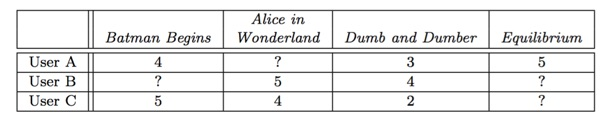
\includegraphics[width=0.75\textwidth]{rm.png}
  \caption{An example of a ratings matrix. Taken from 'Collaborative Filtering Recommender Systems' by Michael D. Ekstrand, John T. Riedl and Joseph A. Konstan.}
\end{figure}

\subsection{Data Splitting}
The data was split by creating a separate ratings matrix, and then removing k entries for each user from the original ratings matrix and adding them to the test ratings matrix. The modified ratings matrix is now the training matrix. \\

\subsection{Calculating similarity}

For the adjusted cosine similarity, I first created a modified ratings matrix, which were normalised by taking the average of each user's ratings and subtracting it from the relevant row in the matrix. The needed vectors were then spliced from this matrix, and the similarity computed using the equation below:

\begin{equation} \label{eq:1}
s(i, j) = \frac{\rbf_i \cdot \rbf_j} {|| \rbf_i ||_2 || \rbf_j ||_2}
\end{equation}

where $\rbf_i$ denotes the normalised vector of ratings for an item, and where each rating is normalised by the average of the user's ratings (i.e via the method above). \\

Unrated items were given the value of 0 so that the vectorised approach could be taken.\\

Due to the vectorised method, for any pair the similarity function compares, if either vector has no ratings, the similarity returns 0. Also, when the euclidian norm is calculated, a check is written in to ensure that the denominator of the function never ends up at 0, returning 0 overall if either is equal to 0.\\

The prediction also has a similar check in to prevent the denominator becoming 0 (which is possible as the predictions may take negative values). \\

The values outputted by the similarity function were in the range [-1, 1]. This made it counter-intuitive to compare to the ratings, as when it was used, the predictions could become negative. To avoid this, the mapping below was used to map the similarities to the range [1, 5].
\begin{equation}
    rescale-similarity(x) = 2x + 3
\end{equation}

In the evaluation stage, the RMSE was calculated for both the scaled and unscaled values.

\subsection{Evaluation}

The RMSE calculation was simply done using two sets of for loops to iterate through the testing matrix. This computationally intense exercise meant that the program took approximately 10 minutes to complete. However, I foresaw no way around this problem, so I merely let the program run its course.\\

\newpage
\section{Project Questions}

\subsection{}
The RMSE on the test set, without the similarity mapping, with k=10 (where k is equal to the number of ratings removed from each user and placed into a separate test set) was approximately equal to 1.442. With the mapping, this value dropped to 0.848. \\

The RMSE on the test set, without the similarity mapping, with k=3 was approximately equal to 1.504. With the mapping, the RMSE dropped to 0.575.\\

Comparing the two unmapped results, one can see that the error increased when decreasing the size of the test set. This may be due to the greater sparsity of the test set giving worse similarity ratings, and therefore less accurate predictions, overall producing less accurate results.\\

In contrast, comparing the mapped results, when k = 10, the set had a larger error than when k = 3. However, both errors significantly dropped from the unmapped values, so it's clear that the similarity mapping was essential. This may be due to the mapping giving the values a more realistic output, and so the predictions and the ratings can be fairly compared.

\subsection{}
This problem is known as the cold-start problem, which results when there isn't enough information about an item to determine what it is similar too - nobody has rated it yet. \\

This problem could be resolved by using hybrid approaches, which uses multiple methods and attributes to recommend content to users, and therefore offsets this problem to some degree. \\

An example of this would be to derive or ask for a user's information, such as the genre of film they enjoy. They could specify this when they initially sign-up for a service, as they have no ratings thus far by which to compare other films. If they have already rated films, the genre of the films they dislike / like can be derived. The system can then give a higher predicted rating for a film with no ratings that is of a genre they like, and a lower predicted rating for a film of a genre they dislike. This would work best in a hybrid approach, with a system like the one implemented here, in order to offset the cold-start problem.

\subsection{}

My solution should scale reasonably well for the bigger datasets, as my adjusted cosine similarity function (which is computationally one of the most complex operations performed) is vectorised, using equation \ref{eq:1}.\\

\texttt{numpy}'s libraries are utilised to perform these operations computationally fast. \\

However, the RMSE calculation has to manually iterate over all the entries in the database, which with k=10 is approximately 10,000 entries, which takes almost 10 minutes to calculate. Therefore this calculation clearly would not scale up to larger datasets.

\newpage
\section{Conclusion}

Overall, my recommender worked well, given the final RMSE ratings. If I were to advance the project further, I would attempt to perform hyper-parameter optimisations over multiple values of k, to see which gives the best RMSE. I also 'sanity checked' my project, by manually looking choosing a movie and guessing roughly how it would be predicted, given the other users who acted similarly. This worked successfully on a few instances.\\

The main stumbling block in the project was the lack of intuitive comprehension of the unmapped values - leading to negative predictions. This was addressed to give a more optimal RMSE, as outlined above. The other small errors, such as 0 indexing, and division-by-0 errors were addressed with simple catch clauses, returning an unrated value. Although this isn't ideal, as this means that some movies may occasionally slip through; due to the precision of the numbers used this is unlikely to happen very often - especially in a dataset of this size. It also, much more importantly, ensures that the program doesn't crash. \\

I would like to test my recommender on a larger dataset, but without access to faster processors or complex parallelisation, it's unlikely to calculate the RMSE in a suitable time.

% \subsection{}
% \nocite{*}
% \printbibliography
\end{document}
